% ------------------------------------------------------------------------
% ICyberPhyS-2026 Beamer presentation
% Source manuscript: Auditable Decision-Making in Intelligent Cyber-Physical
% Systems Using Semantic Transition and Rough Sets
% ------------------------------------------------------------------------

\documentclass[aspectratio=169,xcolor=dvipsnames]{beamer}
\usetheme{KhNU}

\usepackage[T1]{fontenc}
\usepackage[utf8]{inputenc}
\usepackage{amsmath}
\usepackage{amssymb}
\usepackage{array}
\usepackage{booktabs}
\usepackage{graphicx}
\usepackage{tabularx}
\usepackage{tikz}
\usetikzlibrary{calc,positioning}

\hypersetup{
  colorlinks=true,
  linkcolor=dexpiBlue,
  urlcolor=dexpiBlue
}

\setbeamertemplate{caption}{\raggedright\insertcaption\par}
\setlength{\tabcolsep}{3pt}
\renewcommand{\arraystretch}{1.16}
\newcolumntype{Y}{>{\raggedright\arraybackslash}X}
\newcolumntype{L}[1]{>{\raggedright\arraybackslash}p{#1}}

\newcommand{\semtra}{SEMTRA}
\newcommand{\wedd}{WEDD}
\newcommand{\awa}{AwA2}
\newcommand{\slidecaption}[1]{\vspace{0.2em}{\scriptsize #1\par}}
\newcommand{\compactitem}{\setlength{\itemsep}{0.35em}}

\newcommand{\orglogostrip}[1][0.34cm]{%
  \includegraphics[height=#1]{assets/logo_icyberphys.jpg}\hspace{0.18cm}%
  
\includegraphics[height=#1]{assets/logo_ceur.png}\hspace{0.18cm}%
  
\includegraphics[height=#1]{assets/logo_khnu.png}\hspace{0.18cm}%
  \includegraphics[height=#1]{assets/logo_fit.jpg}\hspace{0.18cm}%
  
\includegraphics[height=#1]{assets/logo_kiis.png}\hspace{0.18cm}%
  
\includegraphics[height=#1]{assets/logo_uses.png}\hspace{0.18cm}%
  
\includegraphics[height=#1]{assets/logo_cs.png}%
}

\addtobeamertemplate{frametitle}{}{%
  \begin{tikzpicture}[remember picture,overlay]
    \node[anchor=north east,inner sep=0pt]
      at ([xshift=-0.30cm,yshift=-0.16cm]current page.north east)
      {\includegraphics[height=0.58cm]{assets/logo_icyberphys.jpg}};
  \end{tikzpicture}%
}

\title{\texorpdfstring{\Large Auditable Decision-Making in Intelligent\\Cyber-Physical Systems Using Semantic\\Transition and Rough Sets}{Auditable Decision-Making in Intelligent Cyber-Physical Systems Using Semantic Transition and Rough Sets}}
\subtitle{\small ICyberPhyS-2026: 3rd International Workshop on Intelligent and CyberPhysical Systems}
\author{\normalsize Pavlo Radiuk \and Oleksander Barmak \and Iurii Krak}
\institute{\tiny Khmelnytskyi National University\\Taras Shevchenko National University of Kyiv\\Glushkov Cybernetics Institute}
\date[July 2, 2026]{\scriptsize July 2, 2026 -- Khmelnytskyi, Ukraine}

\begin{document}

% 1
\begin{frame}[plain]
  \titlepage
\end{frame}

% 2
\begin{frame}{Presentation Map}
\small
\tableofcontents
\vfill
{\orglogostrip[0.55cm]\par}
\end{frame}

\section{Motivation}

% 3
\begin{frame}{Why Auditing Is Needed}
\small
\begin{columns}[T,onlytextwidth]
\column{0.48\textwidth}
\begin{block}{CPS safety gap}
\small
\begin{itemize}\compactitem
  \item Deep controllers are accurate but opaque.
  \item Local XAI artifacts do not provide reusable global decision logic.
  \item Safety-critical systems need verifiable reasoning and failsafe behavior.
\end{itemize}
\end{block}
\column{0.48\textwidth}
\begin{alertblock}{Study goal}
\small
Translate latent neural features into explicit, conflict-aware symbolic rulebooks without retraining the underlying controller.
\end{alertblock}
\end{columns}
\vspace{0.4em}
{\scriptsize Keywords: Explainable AI, cyber-physical systems, rough sets, model auditing, production rules, semantic transition.\par}
\end{frame}

% 4
\begin{frame}{Core Contributions}
\small
\begin{columns}[T,onlytextwidth]
\column{0.31\textwidth}
\begin{block}{1. Transition}
\small
Linear transition matrix maps compressed deep representations into physically interpretable semantic attributes.
\end{block}
\column{0.31\textwidth}
\begin{block}{2. Discretization}
\small
\wedd{} balances entropy reduction with local density to convert continuous signals into robust symbolic states.
\end{block}
\column{0.31\textwidth}
\begin{block}{3. Rulebook}
\small
Rough-set induction creates a global rulebook with explicit conflicts, boundary regions, and abstentions.
\end{block}
\end{columns}
\vspace{0.5em}
{\scriptsize The framework acts as a non-destructive post-hoc audit layer for existing neural controllers.\par}
\end{frame}

% 5
\begin{frame}{Position Relative to Prior Work}
\small
\begin{columns}[T,onlytextwidth]
\column{0.48\textwidth}
\begin{block}{What existing methods provide}
\small
\begin{itemize}\compactitem
  \item Local saliency and attribution support model inspection.
  \item Concept bottlenecks align activations with human variables.
  \item Decision trees and rule learners provide symbolic branches.
\end{itemize}
\end{block}
\column{0.48\textwidth}
\begin{alertblock}{What remains missing}
\small
\begin{itemize}\compactitem
  \item Discrete symbolic layer for global logical reasoning.
  \item Formal abstention when evidence is contradictory.
  \item Auditable bridge from neural features to CPS-relevant semantics.
\end{itemize}
\end{alertblock}
\end{columns}
\end{frame}

\section{Method}

% 6
\begin{frame}{SEMTRA Pipeline}
\small
\begin{columns}[T,onlytextwidth]
\column{0.64\textwidth}
\centering
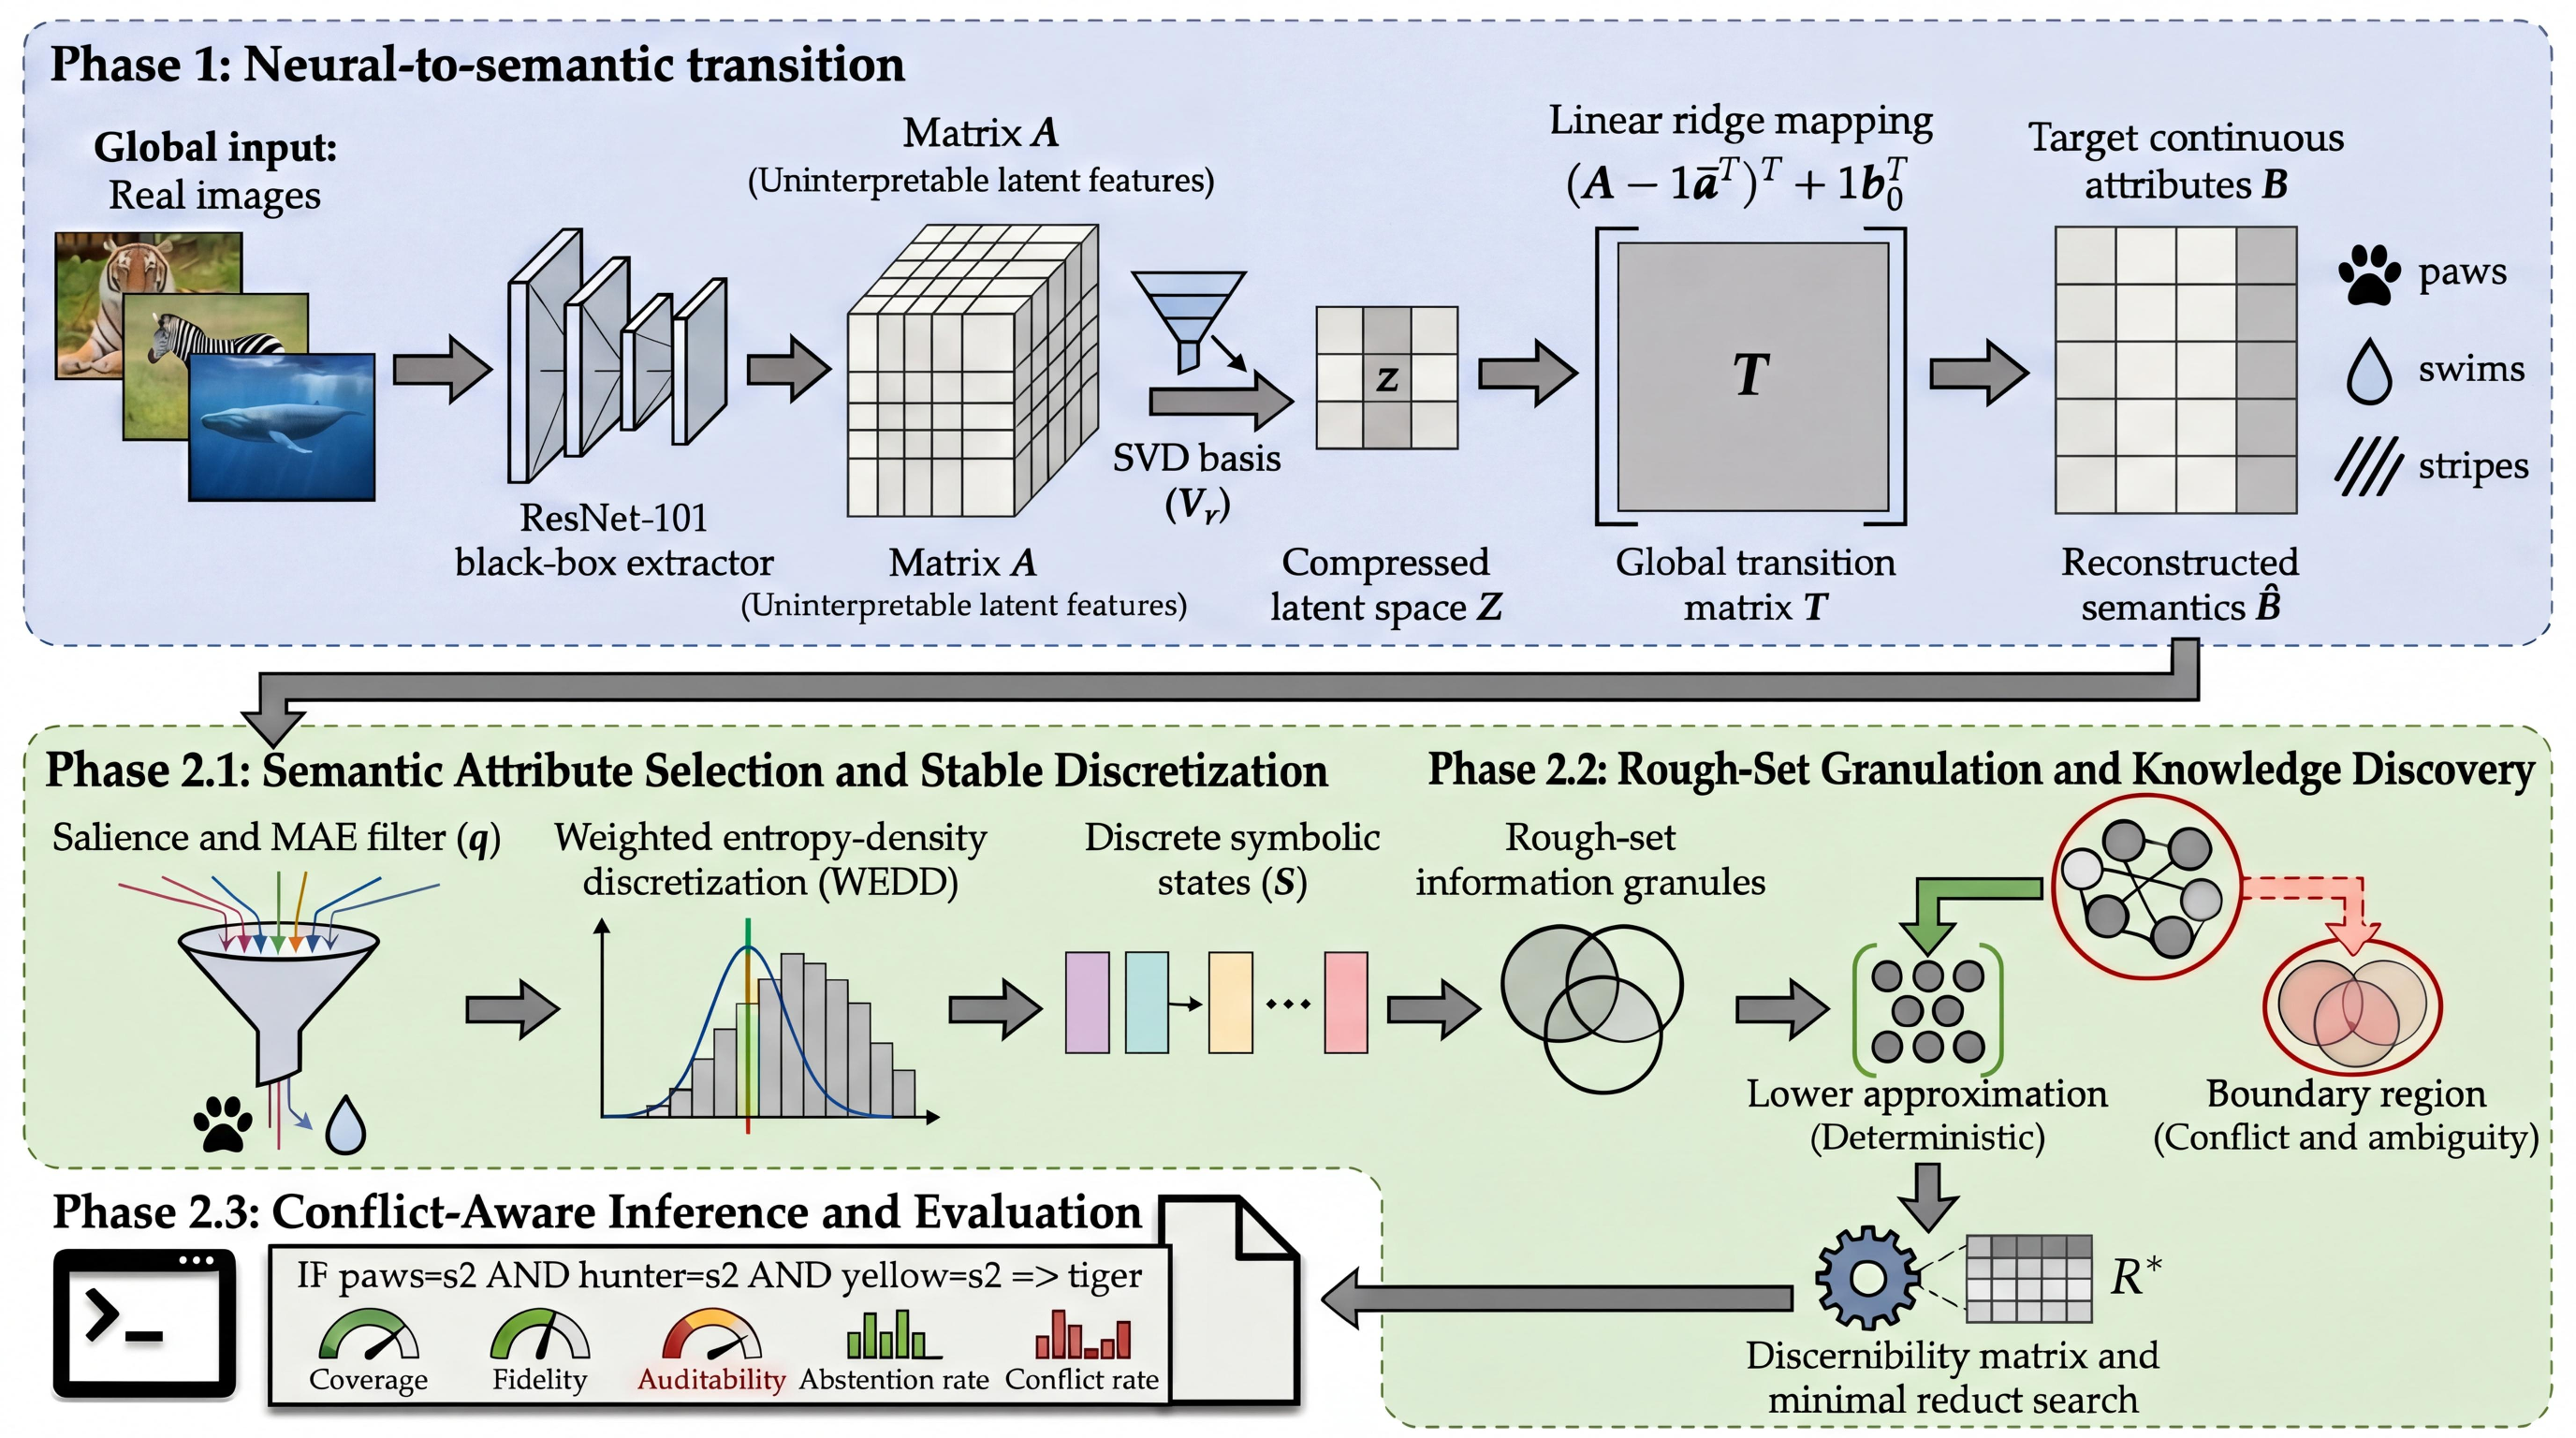
\includegraphics[width=\linewidth,height=0.67\textheight,keepaspectratio]{assets/fig1-semtra-architecture.pdf}
\slidecaption{\textbf{Figure 1:} Conceptual SEMTRA architecture: from the latent space of a neural network to a verified rulebook.}
\column{0.32\textwidth}
\begin{block}{Two-stage audit layer}
\small
\begin{itemize}\compactitem
  \item Frozen neural feature extractor.
  \item Neural-to-semantic transformation.
  \item Semantic-to-symbol granulation.
  \item Rulebook plus audit trace.
\end{itemize}
\end{block}
\end{columns}
\end{frame}

% 7
\begin{frame}{Phase 1: Neural-to-Semantic Transition}
\small
\begin{columns}[T,onlytextwidth]
\column{0.50\textwidth}
\begin{block}{Ridge transition operator}
\small
\[
  A\in\mathbb{R}^{m\times k},\qquad B\in\mathbb{R}^{m\times l}
\]
\[
  T = (A^\top A+\alpha I)^{-1}A^\top B
\]
\end{block}
\column{0.46\textwidth}
\begin{block}{Why it is auditable}
\small
\begin{itemize}\compactitem
  \item Each weight links latent evidence to a semantic attribute.
  \item The base controller remains frozen.
  \item Engineers can inspect which features drive physical meanings.
\end{itemize}
\end{block}
\end{columns}
\vspace{0.25em}
{\scriptsize The manuscript reports this as the bridge between latent space and physically meaningful semantic variables.\par}
\end{frame}

% 8
\begin{frame}{Phase 2.1: Stable Discretization (WEDD)}
\small
\begin{columns}[T,onlytextwidth]
\column{0.54\textwidth}
\begin{block}{Equation (1): threshold objective}
\small
\[
  J_j(\theta)=
  \lambda_H\widetilde{H}_j(\theta)+
  (1-\lambda_H)\widetilde{p}_j(\theta)
  \tag{1}
\]
\end{block}
{\scriptsize \(\widetilde{H}_j(\theta)\) is information entropy; \(\widetilde{p}_j(\theta)\) is a local density proxy estimated with KDE.\par}
\column{0.42\textwidth}
\begin{exampleblock}{Design effect}
\small
\begin{itemize}\compactitem
  \item Thresholds move toward sparse semantic regions.
  \item Micro-perturbations are less likely to change symbolic state.
  \item The resulting states are suitable for rough-set granulation.
\end{itemize}
\end{exampleblock}
\end{columns}
\end{frame}

% 9
\begin{frame}{Phase 2.2: Knowledge Granulation}
\small
\begin{columns}[T,onlytextwidth]
\column{0.54\textwidth}
\begin{block}{Equation (2): induced production rule}
\small
\[
  r:\bigwedge_{j\in R_r}\left[s_j=v_j\right]\Rightarrow d=y_r.
  \tag{2}
\]
\end{block}
{\scriptsize Objects with identical semantic signatures but different classes form boundary regions.\par}
\column{0.42\textwidth}
\begin{block}{Compact audit artifact}
\small
\begin{itemize}\compactitem
  \item Indiscernibility relation over discretized states.
  \item Lower approximation induces reliable rules.
  \item Minimal reducts preserve logic with fewer attributes.
\end{itemize}
\end{block}
\end{columns}
\end{frame}

% 10
\begin{frame}{Conflict-Aware Inference and Auditing}
\small
\begin{columns}[T,onlytextwidth]
\column{0.45\textwidth}
\begin{alertblock}{Honest silence}
\scriptsize
\begin{itemize}\compactitem
  \item Conflict: activated rules disagree.
  \item Abstention: no reliable rule applies.
  \item CPS response: failsafe or human review.
\end{itemize}
\end{alertblock}
\vspace{-0.2em}
\begin{block}{Aggregate support score}
\scriptsize
\resizebox{0.92\linewidth}{!}{$
  S(y_k)=\sum_{r\in\mathcal{A}(x),\,y_r=y_k}\mathrm{conf}(r)\,\mathrm{supp}(r)
$}
\end{block}
\column{0.51\textwidth}
\centering
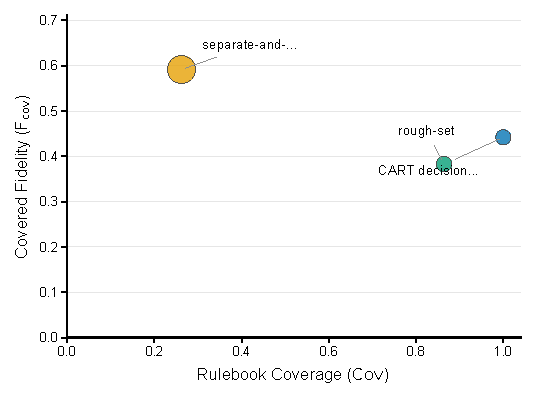
\includegraphics[width=\linewidth,height=0.52\textheight,keepaspectratio]{assets/fig2-coverage-fidelity.pdf}
\slidecaption{\textbf{Figure 2:} Trade-off between rulebook coverage and fidelity. SEMTRA occupies a high-coverage region while explicitly reporting conflicts.}
\end{columns}
\end{frame}

\section{Experimental Results}

% 11
\begin{frame}{Semantic-Space Reconstruction}
\small
\begin{block}{AwA2 Protocol A}
\small
The evaluation uses Animals with Attributes 2: 50 object classes described by 85 semantic attributes, averaged across five seeds.
\end{block}
\vspace{0.25em}
{\scriptsize \textbf{Table 1:} AwA2 Protocol A transition reconstruction metrics. Metrics are reported as mean \(\pm\) standard deviation across five seeds.\par}
\vspace{0.15em}
\scriptsize
\begin{tabularx}{\linewidth}{lccc}
\toprule
\textbf{Split} & \textbf{MAE} & \textbf{RMSE} & \textbf{Mean semantic correlation}\\
\midrule
train & \(0.1027\pm0.0003\) & \(0.1482\pm0.0004\) & \(0.8079\pm0.0009\)\\
validation & \(0.1030\pm0.0003\) & \(0.1486\pm0.0005\) & \(0.8065\pm0.0014\)\\
test & \(0.1029\pm0.0005\) & \(0.1484\pm0.0007\) & \(0.8070\pm0.0018\)\\
\bottomrule
\end{tabularx}
\vspace{0.25em}
{\scriptsize Test MAE \(=0.1029\) and correlation \(=0.8070\) show a stable neural-to-semantic bridge.\par}
\end{frame}

% 12
\begin{frame}{Rulebook Properties and Audit Tax}
\small
{\scriptsize \textbf{Table 2:} General rulebook properties and symbolic-baseline comparison. Point estimates are reported alongside standard deviations over five random seeds for the proposed method.\par}
\vspace{0.15em}
\scriptsize
\begin{tabularx}{\linewidth}{Yccc}
\toprule
\textbf{Metric} & \textbf{Value (ours)} & \textbf{CART baseline} & \textbf{Separate-and-conquer}\\
\midrule
Number of rules & \(59.00\pm2.55\) & 53 & 197\\
Test coverage & \(0.8480\pm0.0530\) & 1.0000 & 0.2620\\
Covered accuracy & \(0.3973\pm0.0109\) & 0.4129 & 0.6334\\
Covered fidelity to base & \(0.4048\pm0.0078\) & -- & --\\
Average conditions per rule & \(4.0397\pm0.0543\) & 7.0000 & 3.2589\\
Test abstention rate & \(0.1520\pm0.0530\) & 0.0000 & 0.7380\\
Test conflict rate & \(0.1375\pm0.0532\) & 0.0000 & 0.2301\\
\bottomrule
\end{tabularx}
\vspace{0.25em}
{\scriptsize The audit tax is the part of model behavior that can be preserved as strict, inspectable predicates.\par}
\end{frame}

% 13
\begin{frame}{Robustness to Semantic Noise}
\small
{\scriptsize \textbf{Table 3:} Synthetic stress-test results averaged over random seeds.\par}
\vspace{0.15em}
\scriptsize
\begin{tabularx}{\linewidth}{lccccc}
\toprule
\textbf{Noise \((\sigma)\)} & \textbf{MAE} & \textbf{Threshold err.} & \textbf{Rule Jaccard} & \textbf{Macro-F1} & \textbf{Coverage}\\
\midrule
0.000 & 0.000 & 0.014 & 0.700 & 0.879 & 0.971\\
0.100 & 0.021 & 0.018 & 0.763 & 0.881 & 0.962\\
0.200 & 0.041 & 0.017 & 0.743 & 0.838 & 0.952\\
\bottomrule
\end{tabularx}
\vspace{0.45em}
\begin{exampleblock}{Result}
\small
\begin{itemize}\compactitem
  \item Macro-F1 remains \(0.838\) at \(\sigma=0.20\).
  \item Coverage remains \(95.2\%\).
  \item WEDD filters small semantic perturbations while preserving inference.
\end{itemize}
\end{exampleblock}
\end{frame}

% 14
\begin{frame}{Representative Production Rules}
\scriptsize
\textbf{Table 4:} Representative induced production rules from AwA2 Protocol A. Support refers to the number of instances covered in the training partition.
\vspace{0.2em}

{\setlength{\tabcolsep}{2.5pt}
\begin{tabularx}{\linewidth}{L{1.35cm}Y Y L{1.65cm}}
\toprule
\textbf{Rule / class} & \textbf{Antecedent} & \textbf{Numeric bounds} & \textbf{Support / Conf.}\\
\midrule
R0001 / tiger & paws=s2 AND hunter=s2 AND small=s0 AND yellow=s2 & paws\(\ge0.40\); hunter\(\ge0.40\); small\(<0.15\); yellow\(\ge0.40\) & 115 / 0.896\\
R0003 / antelope & stripes=s1 AND hooves=s3 AND paws=s0 AND hands=s0 AND small=s1 AND yellow=s1 & stripes\(\in[0.15,0.40]\); hooves\(\ge0.70\); paws\(<0.15\); hands\(<0.15\); small\(\in[0.15,0.40]\); yellow\(\in[0.15,0.40]\) & 132 / 0.871\\
R0004 / zebra & hunter=s0 AND water=s0 AND small=s0 AND jungle=s2 AND yellow=s1 & hunter\(<0.15\); water\(<0.15\); small\(<0.15\); jungle\(\ge0.40\); yellow\(\in[0.15,0.40]\) & 434 / 0.866\\
\bottomrule
\end{tabularx}
}
\vspace{0.25em}
{\scriptsize Each rule is inspectable against physical or semantic sensor specifications.\par}
\end{frame}

% 15
\begin{frame}{Semantic Attribute Diagnostics}
\small
\begin{columns}[T,onlytextwidth]
\column{0.49\textwidth}
\centering
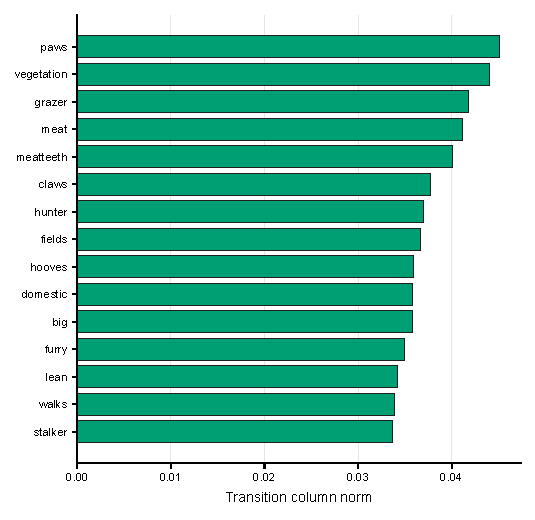
\includegraphics[width=\linewidth,height=0.55\textheight,keepaspectratio]{assets/fig3a-semantic-diagnostics.pdf}
{\scriptsize (a) Transition salience by semantic attribute.\par}
\column{0.49\textwidth}
\centering
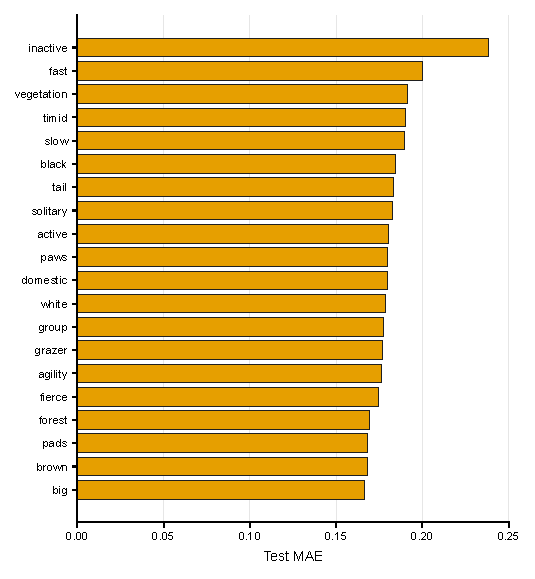
\includegraphics[width=\linewidth,height=0.55\textheight,keepaspectratio]{assets/fig3b-semantic-diagnostics.pdf}
{\scriptsize (b) Attribute-wise semantic reconstruction error on AwA2.\par}
\end{columns}
\slidecaption{\textbf{Figure 3:} Semantic attribute diagnostics: (a) transition salience by semantic attribute; (b) attribute-wise semantic reconstruction error on AwA2.}
{\scriptsize High-salience attributes such as paws and vegetation reveal which physical features dominate model logic.\par}
\end{frame}

% 16
\begin{frame}{Threshold Optimization Dashboard}
\small
\begin{columns}[T,onlytextwidth]
\column{0.61\textwidth}
\centering
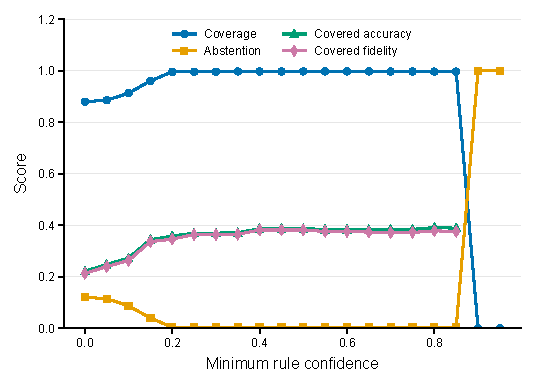
\includegraphics[width=\linewidth,height=0.63\textheight,keepaspectratio]{assets/fig4-threshold-optimization.pdf}
\slidecaption{\textbf{Figure 4:} Rulebook and threshold optimization. Coverage, abstention, covered accuracy, and covered fidelity as the minimum rule-confidence threshold varies.}
\column{0.35\textwidth}
\begin{block}{Operational tuning}
\small
\begin{itemize}\compactitem
  \item Lower threshold: more autonomous coverage.
  \item Higher threshold: stricter human oversight.
  \item The dashboard exposes the coverage-abstention trade-off directly.
\end{itemize}
\end{block}
\end{columns}
\end{frame}

% 17
\begin{frame}{Inference Traces}
\scriptsize
\textbf{Table 5:} Representative rule inference traces with object ID, prediction, matched-rule evidence, and antecedent states.
\vspace{0.2em}

{\setlength{\tabcolsep}{2.5pt}
\begin{tabularx}{\linewidth}{L{2.1cm}L{2.4cm}L{2.4cm}Y}
\toprule
\textbf{Case / object} & \textbf{True / pred. / mode} & \textbf{Rule evidence} & \textbf{Antecedent states}\\
\midrule
correct exact / 5083 & collie / collie / exact & R0027; support 1675; conf. 0.208 & stripes=s0; hooves=s0; swims=s1; paws=s3; longneck=s0; hunter=s1; ocean=s1; quadrapedal=s3\\
abstention / 24024 & ox / abstain / exact & R0029; support 2820; conf. 0.195 & stripes=s0; hooves=s2; swims=s1; paws=s0; longneck=s1; hunter=s0; ocean=s1; quadrapedal=s2\\
fallback error or boundary / 16781 & hamster / mole / fallback & no matched rule; boundary evidence & stripes=s0; hooves=s1; swims=s1; paws=s2; longneck=s0; hunter=s0; ocean=s1; quadrapedal=s2\\
\bottomrule
\end{tabularx}
}
\vspace{0.25em}
{\scriptsize The trace shows whether an error comes from sensor evidence, boundary matching, or conflict in the knowledge base.\par}
\end{frame}

\section{Discussion}

% 18
\begin{frame}{Implications for Intelligent CPS}
\small
\begin{columns}[T,onlytextwidth]
\column{0.32\textwidth}
\begin{block}{Transparent twin}
\small
\semtra{} builds a symbolic digital twin of model logic aligned with trustworthy-AI accountability needs.
\end{block}
\column{0.32\textwidth}
\begin{block}{Failsafe signal}
\small
Detected conflicts \(13.75\%\) and abstentions \(15.20\%\) become explicit triggers for halt or human review.
\end{block}
\column{0.32\textwidth}
\begin{block}{Legacy retrofit}
\small
The method runs post hoc on frozen feature extractors, avoiding expensive controller retraining.
\end{block}
\end{columns}
\vspace{0.35em}
{\scriptsize The covered-fidelity score of \(40.48\%\) quantifies how much neural behavior is preserved as certifiable symbolic logic.\par}
\end{frame}

% 19
\begin{frame}{Limitations and Future Work}
\small
\begin{columns}[T,onlytextwidth]
\column{0.48\textwidth}
\begin{alertblock}{Current limitations}
\small
\begin{itemize}\compactitem
  \item Static, manually annotated semantic dictionaries.
  \item Parallel diagnostic tool, not a full neural-network replacement.
  \item Interpretability requires accepting the audit tax.
\end{itemize}
\end{alertblock}
\column{0.48\textwidth}
\begin{exampleblock}{Next steps}
\small
\begin{itemize}\compactitem
  \item Automated concept discovery.
  \item Dynamic construction of attribute spaces.
  \item LLM-assisted semantic representation generation for changing industrial environments.
\end{itemize}
\end{exampleblock}
\end{columns}
\end{frame}

% 20
\begin{frame}{Contact}
\normalsize
\begin{columns}[T,onlytextwidth]
\column{0.52\textwidth}
\begin{block}{Authors}
\small
Pavlo Radiuk\\
Oleksander Barmak\\
Iurii Krak
\end{block}
\begin{block}{Correspondence}
\small
\href{mailto:radiukp@khmnu.edu.ua}{radiukp@khmnu.edu.ua}\\
\href{mailto:barmako@khmnu.edu.ua}{barmako@khmnu.edu.ua}\\
\href{mailto:iurii.krak@knu.ua}{iurii.krak@knu.ua}
\end{block}
\column{0.42\textwidth}
\begin{block}{Affiliations}
\small
Khmelnytskyi National University\\
Taras Shevchenko National University of Kyiv\\
Glushkov Cybernetics Institute
\end{block}
\vspace{0.7em}
{\scriptsize\orglogostrip\par}
\end{columns}
\vfill
{\scriptsize ICyberPhyS-2026, Khmelnytskyi, Ukraine.\par}
\end{frame}

\end{document}
